\chapter{RESULTS AND ANALYSIS}

A comparative evaluation of active and passive band-pass filter topologies was conducted for the analog input stage of a MEMS microphone audio acquisition system. The target passband was 100 Hz to 3.4 kHz, and the magnitude response of each filter was measured directly from FFT acquisitions.

The measured gain values (in dB) are summarised in the following table.

\begin{table}[H]
\caption{Measured Gain of Active and Passive Band-Pass Filters}
\label{tab:gain_comparison}
\renewcommand{\arraystretch}{1.4}

\begin{tabularx}{\textwidth}
{|
>{\centering\arraybackslash}Y|
>{\centering\arraybackslash}Y|
>{\centering\arraybackslash}Y|}

\hline
\textbf{Frequency (Hz)} & \textbf{Active Filter Gain (dB)} & \textbf{Passive Filter Gain (dB)} \\
\hline

80   & $-16.0$ & $-22.4$ \\
\hline
120  & $-15.2$ & $-16.0$ \\
\hline
160  & $-7.2$  & $-11.2$ \\
\hline
320  & $-1.6$  & $-4.8$ \\
\hline
440  & $-1.6$  & $-7.2$ \\
\hline
520  & $-2.4$  & $-6.4$ \\
\hline
600  & $+1.6$  & $-3.2$ \\
\hline
800  & $-0.8$  & $-5.6$ \\
\hline
1200 & $-0.8$  & $-5.6$ \\
\hline
2000 & $0.0$   & $-5.6$ \\
\hline
2800 & $-3.2$  & $-6.4$ \\
\hline
3200 & $-3.2$  & $-6.4$ \\
\hline
4000 & $-6.4$  & -- \\
\hline

\end{tabularx}
\end{table}

The active filter exhibited a flat in-band response, with gain remaining within $\pm$1.6 dB from 320 Hz to 2 kHz and falling only to -3.2 dB at the upper edge of the band. In contrast, the passive filter demonstrated substantial attenuation throughout the entire passband, with the peak gain at 600 Hz reaching only -3.2 dB and typical levels between -4.8 and -7.2 dB across most of the band. This significant loss of signal energy would degrade the signal-to-noise ratio and push the microphone output below the optimal range of the following analogue-to-digital converter, necessitating an additional preamplifier stage and increasing overall system complexity.

The frequency responses of both designed filters have been visualized below:

\begin{figure}[H]
    \centering
    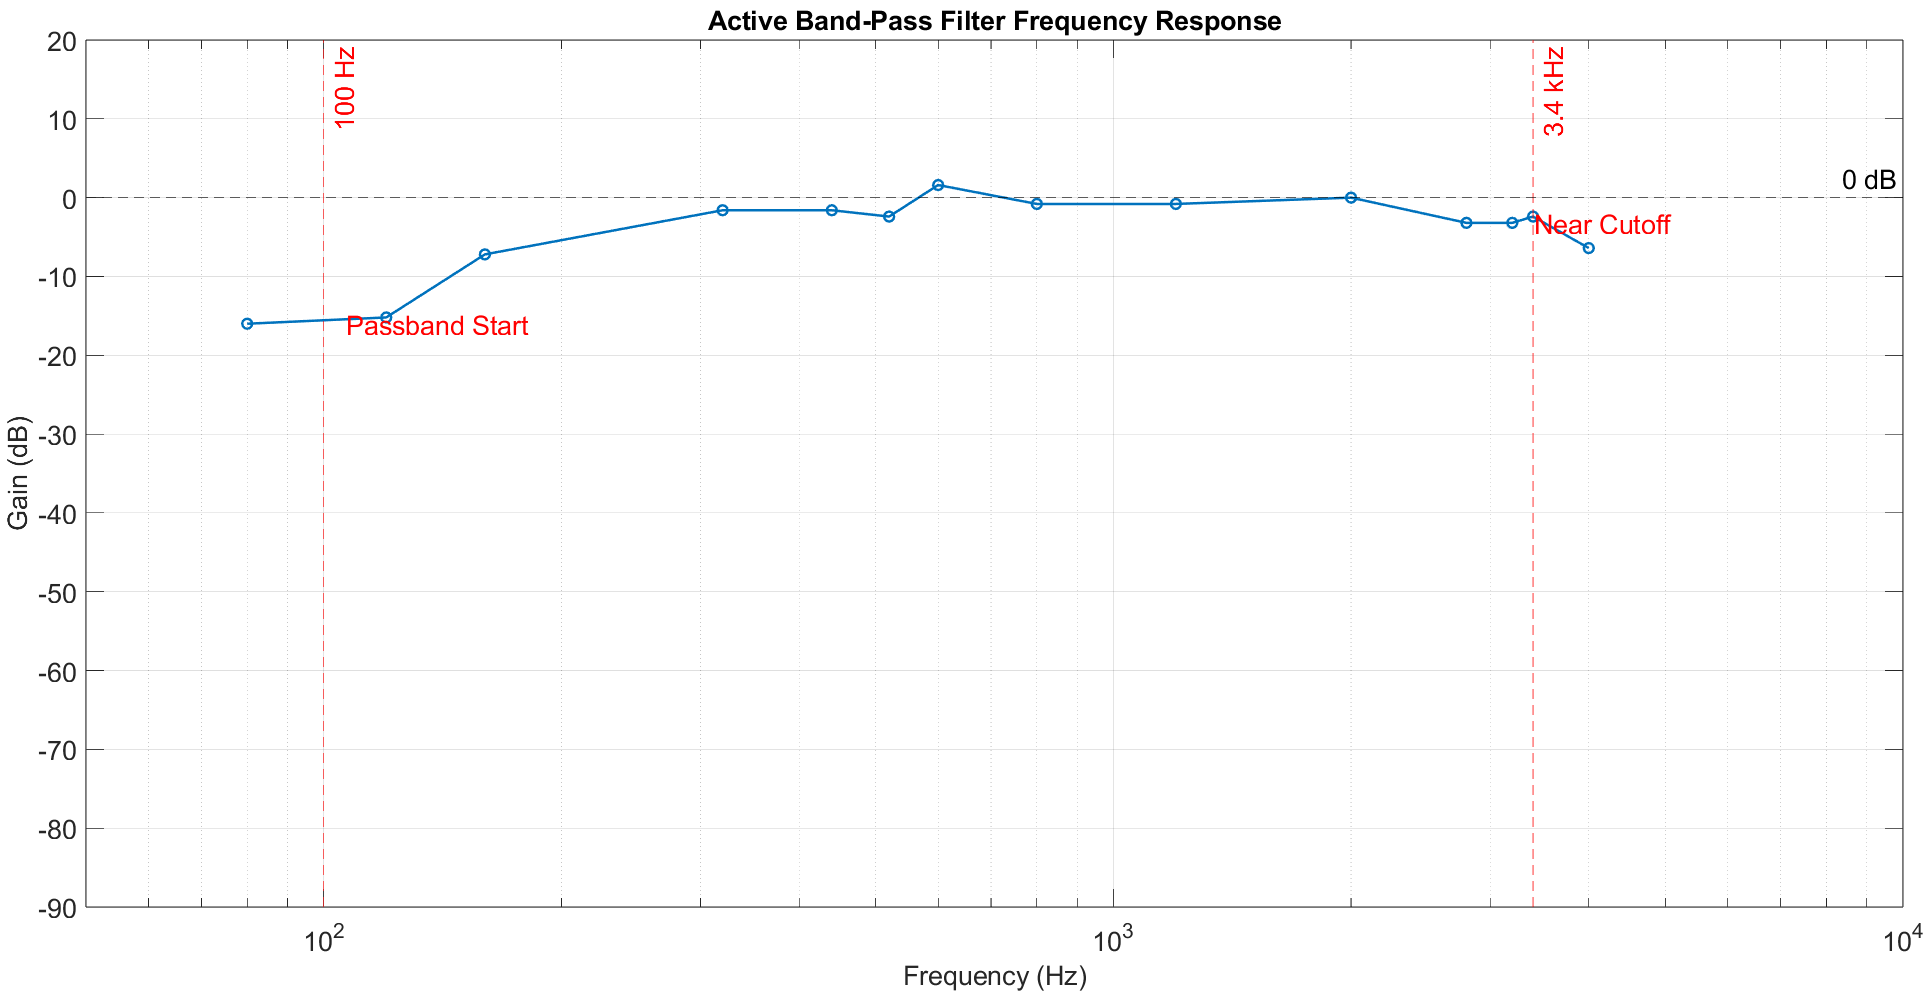
\includegraphics[width=1\linewidth]{src/images/Filter_2_op_amp.png}
    \caption{Active Band-Pass Filter Frequency Response}
    \label{fig:2_op_amp_filter}
\end{figure}

\begin{figure}[H]
    \centering
    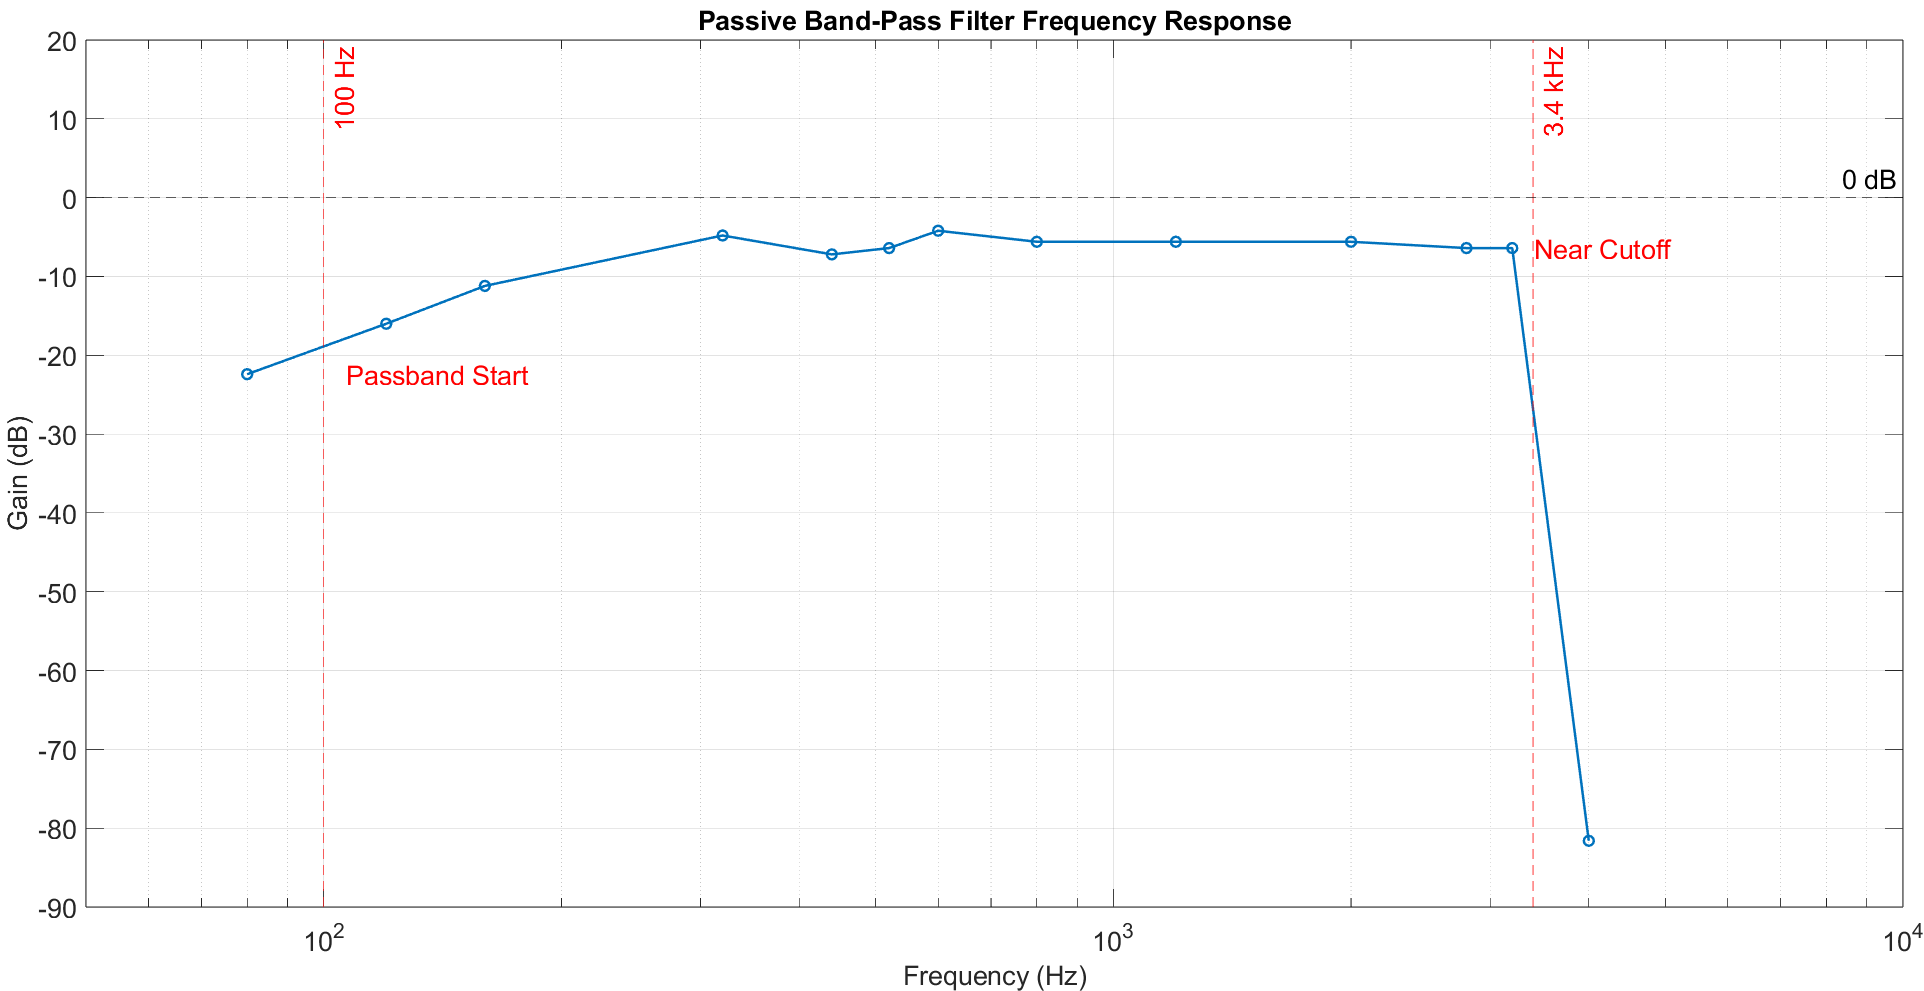
\includegraphics[width=1\linewidth]{src/images/passive_filter.png}
    \caption{Passive Band-Pass Filter Frequency Response}
    \label{fig:passive_filter}
\end{figure}

Based on these results, the passive topology is considered sub-optimal for this application. While the tested single-stage active filter provides a flat, near-unity response across the band, it does not offer significant passband gain or steep roll-off outside the transition region. To address these requirements, a four-stage Sallen-Key active filter topology will be implemented in the final design, providing both increased passband gain and improved stopband attenuation. This approach will ensure robust signal conditioning and enhanced rejection of out-of-band noise for the MEMS microphone input stage.